\documentclass[dvipsnames]{beamer}\usepackage[]{graphicx}\usepackage[]{color}
%% maxwidth is the original width if it is less than linewidth
%% otherwise use linewidth (to make sure the graphics do not exceed the margin)
\makeatletter
\def\maxwidth{ %
  \ifdim\Gin@nat@width>\linewidth
    \linewidth
  \else
    \Gin@nat@width
  \fi
}
\makeatother

\definecolor{fgcolor}{rgb}{0.345, 0.345, 0.345}
\newcommand{\hlnum}[1]{\textcolor[rgb]{0.686,0.059,0.569}{#1}}%
\newcommand{\hlstr}[1]{\textcolor[rgb]{0.192,0.494,0.8}{#1}}%
\newcommand{\hlcom}[1]{\textcolor[rgb]{0.678,0.584,0.686}{\textit{#1}}}%
\newcommand{\hlopt}[1]{\textcolor[rgb]{0,0,0}{#1}}%
\newcommand{\hlstd}[1]{\textcolor[rgb]{0.345,0.345,0.345}{#1}}%
\newcommand{\hlkwa}[1]{\textcolor[rgb]{0.161,0.373,0.58}{\textbf{#1}}}%
\newcommand{\hlkwb}[1]{\textcolor[rgb]{0.69,0.353,0.396}{#1}}%
\newcommand{\hlkwc}[1]{\textcolor[rgb]{0.333,0.667,0.333}{#1}}%
\newcommand{\hlkwd}[1]{\textcolor[rgb]{0.737,0.353,0.396}{\textbf{#1}}}%

\usepackage{framed}
\makeatletter
\newenvironment{kframe}{%
 \def\at@end@of@kframe{}%
 \ifinner\ifhmode%
  \def\at@end@of@kframe{\end{minipage}}%
  \begin{minipage}{\columnwidth}%
 \fi\fi%
 \def\FrameCommand##1{\hskip\@totalleftmargin \hskip-\fboxsep
 \colorbox{shadecolor}{##1}\hskip-\fboxsep
     % There is no \\@totalrightmargin, so:
     \hskip-\linewidth \hskip-\@totalleftmargin \hskip\columnwidth}%
 \MakeFramed {\advance\hsize-\width
   \@totalleftmargin\z@ \linewidth\hsize
   \@setminipage}}%
 {\par\unskip\endMakeFramed%
 \at@end@of@kframe}
\makeatother

\definecolor{shadecolor}{rgb}{.97, .97, .97}
\definecolor{messagecolor}{rgb}{0, 0, 0}
\definecolor{warningcolor}{rgb}{1, 0, 1}
\definecolor{errorcolor}{rgb}{1, 0, 0}
\newenvironment{knitrout}{}{} % an empty environment to be redefined in TeX

\usepackage{alltt}
\usepackage{color} % for colors
\usepackage{graphicx}
\usepackage{hyperref}
\usepackage{svg}
\hypersetup{
    bookmarks=true,         % show bookmarks bar?
    unicode=false,          % non-Latin characters in Acrobat?s bookmarks
    pdftoolbar=true,        % show Acrobat?s toolbar?
    pdfmenubar=true,        % show Acrobat?s menu?
    pdffitwindow=false,     % window fit to page when opened
    pdfstartview={FitH},    % fits the width of the page to the window
    pdftitle={My title},    % title
    pdfauthor={Author},     % author
    pdfsubject={Subject},   % subject of the document
    pdfcreator={Creator},   % creator of the document
    pdfproducer={Producer}, % producer of the document
    pdfkeywords={keyword1} {key2} {key3}, % list of keywords
    pdfnewwindow=true,      % links in new PDF window
    colorlinks=true,       % false: boxed links; true: colored links
    linkcolor=red,          % color of internal links (change box color with linkbordercolor)
    citecolor=green,        % color of links to bibliography
    filecolor=magenta,      % color of file links
    urlcolor=blue         % color of external links
}
% \usepackage{beamerthemesplit} // Activate for custom appearance
\beamertemplatenavigationsymbolsempty

\definecolor{wapurple}{HTML}{433447}
\definecolor{wared}{HTML}{D16B54}

\usecolortheme{beaver}
\title{E-411-PRMA}
\subtitle{Lecture 3}
\author{Christopher David Desjardins}
\date{24 August 2015}
\IfFileExists{upquote.sty}{\usepackage{upquote}}{}
\begin{document}






\begin{frame}
\frametitle{This week}
\begin{itemize}
  \item Classical test theory
  \item Reliability
\end{itemize}
\end{frame}

{
\setbeamercolor{normal text}{bg=RoyalBlue}
\begin{frame}
\centering
\begin{itemize}
\item[]<1-> \Huge \textcolor{white}{Is there a perfect or exact measurement?}
                           
\vspace{1cm}
\item[]<2->\Huge \textcolor{white}{Must we always deal with error?}
\end{itemize}
\end{frame}
}

\begin{frame}
\frametitle{Dealing with imperfect measurements}
\begin{itemize}
  \item Error is part of a measurement
  \item Minimize error 
  \item Partition out error 
\end{itemize}
\end{frame}

\begin{frame}
\frametitle{Introduction to classical test theory}
From Rodriguez (2015)\footnotemark 
\begin{enumerate}
  \item<1->No single approach to the measurement of any construct is universally accepted.
\item<2->Psychological measurements are usually based on limited samples of behavior.
\item<3->The measurement obtained is always subject to error.
\item<4->The lack of well-defined units on the measurement scales poses still another problem.
\item<5->Psychological constructs cannot be defined only in terms of operational definitions but must also have demonstrated relationships to other constructs or observable phenomena
\end{enumerate}
\footnotetext{source: \url{http://edmeasurement.net/resources/Introctt.html}}
\end{frame}

\begin{frame}
\frametitle{Intro to CTT, con't}
From Rodriguez, 2015:

\vspace{1cm}
Classical test theory provides a \textbf{model} for us to \textbf{understand}, \textbf{manipulate}, and \textbf{interpret} our \textbf{measurements}.  It is a model based on the idea that \textbf{observations}, made through any process, are \textbf{not} absolute or \textbf{perfect}.  There is \textbf{error} to varying degrees \textbf{in our observations} or measurements.  The \textbf{classical test theory model} gives us a way to \textbf{understand} the role of \textbf{error}, its \textbf{sources}, and ways to \textbf{estimate} its \textbf{impact} on our \textbf{measurements} and our \textbf{interpretations}. 
\end{frame}

\begin{frame}
\frametitle{CTT model}

\begin{center}
$$ \underbrace{X}_{\text{observed score}} = \underbrace{T}_{\text{true score}} + \underbrace{E}_{\text{error}} $$
\end{center}

\begin{itemize}
\item<2-> If we give a test to measure depression, what is the depression score we get? X or T?
\item<3-> Do we ever observe T?
\item<4-> T is stable
\item<5-> CTT looks similar to simple linear regression
  \begin{itemize}
    \item<6-> Height = Weight + Error
    \item<7-> However, T is latent and our unknown variable
  \end{itemize}
\end{itemize}
\end{frame}

\begin{frame}
\centering
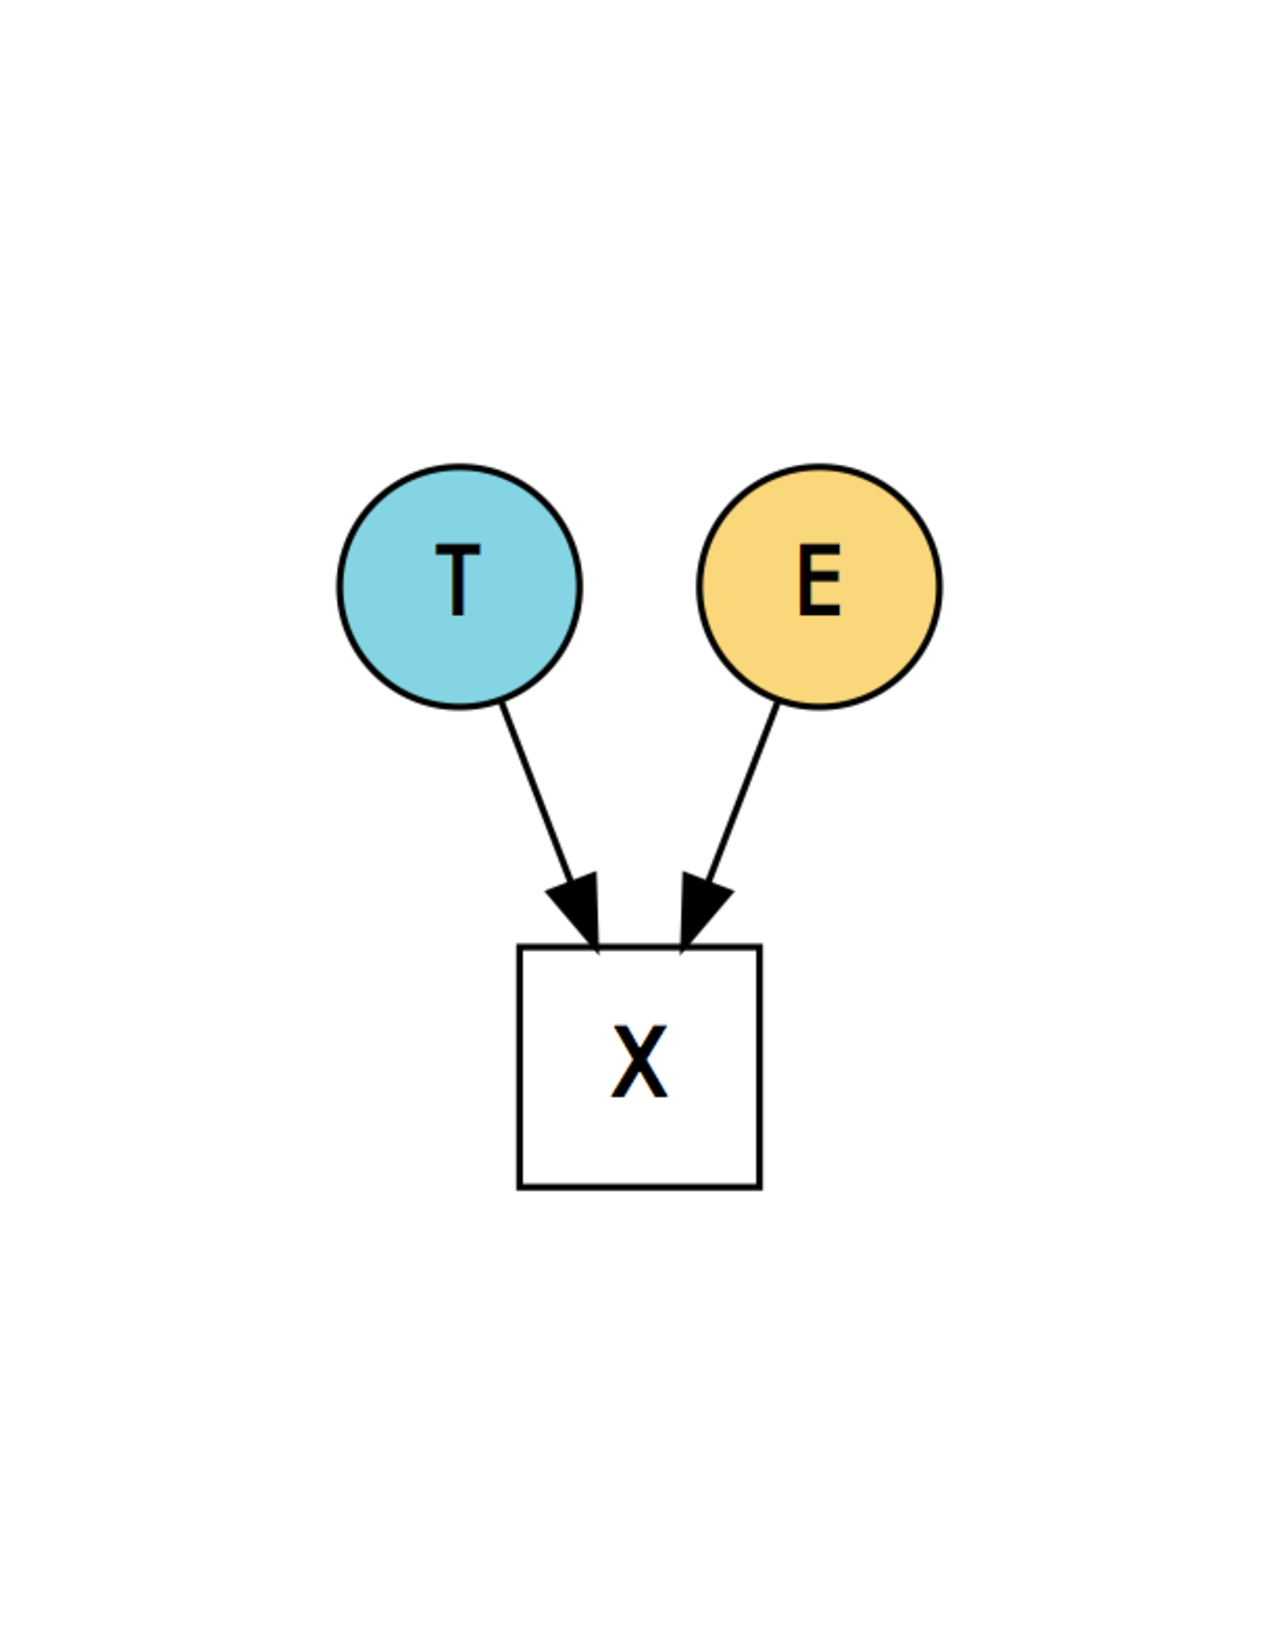
\includegraphics[trim = 0 0 0 130, clip = T, scale = .5]{images/ctt.pdf}


\end{frame}

\begin{frame}
\frametitle{Variance}
\begin{itemize}
  \item<1-> Recall: Variance is a measure of variability
  \item<2-> Recall: Standard deviation is the square root of variance
  \item[]<3->\centering $\frac{\sum(Y - \bar{Y})^2}{N} $
  \item<4-> Sum of squared differences, distance an observation is from the mean, divided by the sample size 
  \item<5-> \textcolor{red}{Very important concept in CTT and measurement!}
  \item<6-> You administer a test and the students get the following grades: 76, 87, 88, 80, 77. Calculate the variance.
  \item<7-> You administer the same test again to other students and they get the following grades: 107, 78, 78, 94, 77. 
  \item<8-> Would you expect that the variance should be the same?
\end{itemize}
\end{frame}

\begin{frame}
\frametitle{Partitioning of variance in CTT}
$$\underbrace{\sigma^2_X}_{\text{Observed Score Variance}} = \underbrace{\sigma^2_T}_{\text{True Score Variance}} + \underbrace{\sigma^2_E}_{\text{Error Variance}}$$
\begin{itemize}
  \item<2-> True score variance is considered to be static (i.e.\ it never changes based on the test)
  \item<3-> What affect does error variance have on ...
    \begin{itemize}
      \item<4-> The consistency of scores?
      \item<5-> The usefulness of test?
      \item<6-> Observed score variance?
    \end{itemize}
\end{itemize}
\end{frame}

{
\setbeamercolor{normal text}{bg=RoyalBlue}
\begin{frame}
\centering
\Huge \textcolor{white}{What goes into error variance?}
\end{frame}
}

\begin{frame}
\frametitle{Sources of measurement error}
\begin{itemize}
\item<1->\textcolor{red}{Random Error}
  \begin{itemize}
  \item<2-> Unpredictable and inconsistent sources of error
  \end{itemize}
\item<3->\textcolor{red}{Systematic Error}
  \begin{itemize}
  \item<4->Constant and predictable source of error
  \end{itemize}
\item<5->Examples of each?
\item<6->Which poses a bigger threat to a
  \begin{itemize} 
    \item<7-> Consistent measure?
    \item<8-> Validity?
    \item<9-> Reliability?
  \end{itemize}
\end{itemize}
\end{frame}

{
\setbeamercolor{normal text}{bg=RoyalBlue}
\begin{frame}
\centering
\Huge \textcolor{white}{What are the sources of error in testing?}
\end{frame}
}

\begin{frame}
\begin{itemize}
  \item Construction
  \item Administration
  \item Scoring
  \item Interpretation
\end{itemize}
\end{frame}

\begin{frame}
\frametitle{Reliability def'n}
$$\text{reliability} = \frac{\overbrace{\sigma^2_T}^{\text{true score variance}}}{\underbrace{\sigma^2_X}_{\text{observed score variance}}}$$

\begin{itemize}
  \item<2-> What is the interpretation?
  \item<3-> What can reliability range from?
  \item<4-> What are estimates of reliability you've heard of??
\end{itemize}
\end{frame}

\begin{frame}
\frametitle{Reliability GIF}
  \url{https://cddesja.github.io/classes/e411prma2015-1/lecture3/images/darts.gif}\footnotemark

  \footnotetext{original source: \href{http://giphy.com/gifs/cheezburger-fail-QINL0oJPaluvK}{Giphy}}
\end{frame}

\begin{frame}
\frametitle{Types of Reliability}
\begin{itemize}
\item <1->Test-Retest
  \begin{itemize}
    \item<1-> \underline{Coefficient of stability}
    \item <1->What are sources of error here?
  \end{itemize}
\item <2->Parallel Forms
  \begin{itemize}
    \item <2->Means and varinces of the test scores are equivalent
    \item <2->\underline{Coefficient of equivalence}
    \item <2->Parallel forms reliability
    \item <2->What are sources of error here?
  \end{itemize}
\item<3-> Alternate Forms 
  \begin{itemize}
    \item<3-> Versions of a test designed to be parallel
    \item<3-> Not necessarily parallel
    \item<3-> \underline{Alternate forms reliability}
  \end{itemize}
\item<4-> Fortunately, we can calculate measures of internal consistency
\end{itemize}
\end{frame}

\begin{frame}
\frametitle{Different types of associations}
\begin{itemize}
  \item Pearson's product-moment correlation only appropriate when variables are continuous and are interval/ratio scales
  \item \textcolor{blue}{Alternatives when variables are dichotomous either naturally or artifically (assumed to have a continuous underlying scale)}
  \begin{itemize}
    \item \textcolor{red}{Phi coefficient}, equivalent to Pearson's correlation but for dichotomous variables
    \item \textcolor{red}{Polychoric coefficient}, an index of association between two artifically ordinal variables
    \item \textcolor{red}{Tetrachoric coefficient}, an index of association between two artifically dichotomized variables
    \item \textcolor{red}{Point-biserial coefficient}, an index of association betweeen a dichotomous and a continous variable
    \item \textcolor{red}{Biserial coefficient}, an index of association betweeen an artificially dichotomous and a continous variable
    \item \textcolor{red}{Spearman Rank-Order coefficient}, an index of association where at least one variable is ordinal
    \item \textcolor{red}{Kendall's tau}, alternative to Spearman
  \end{itemize}
\end{itemize}
\end{frame}

\begin{frame}
\frametitle{Internal consistency}
  \begin{itemize}
    \item<1-> Measure level of consistency or agreement between items
    \item<2-> A test is unidimensional if all the items measure the same latent construct
    \item<3-> The more items measure just one construct, the higher the internal consistency
    \item<4-> Is it always possible or desirable to have a test that measures just one thing?
  \end{itemize}
\end{frame}

\begin{frame}
  \frametitle{Split-Half Reliability}
  \begin{itemize}
    \item Obtained by correlating (Pearson's coefficient) two pairs of scores from equivalent halves of a single test then apply a correction
    \item Creating two equivalent forms of a test
    \begin{itemize}
    \item \textcolor{wapurple}{What are the steps to calculate a split-half reliability?}
    \item \textcolor{wapurple}{How might we consider making splits?}
    \item \textcolor{wapurple}{What do we need to be careful of?}
    \end{itemize}
  \end{itemize}
\end{frame}

\begin{frame}
  \frametitle{Why a correction?}
  \begin{itemize}
    \item<1-> \textcolor{wared}{Uncorrected reliability is biased downward}
    \begin{itemize}
      \item<2-> Measurement error
      \item<2-> Range restriction
    \end{itemize}
    \item<3-> \textcolor{wared}{Which should have higher reliability?}
      \begin{itemize}
        \item Test A, a math test consisting of math problems and word problems, or Test B, a math test consisting of just math problems?
        \item Test C, which is 25 items long, or Test D, which is 50 items long?
        \item Test E, which is a timed test, or Test F, which is the same test as E but you can take as long as you need on the test?
      \end{itemize}
    \end{itemize}
\end{frame}

\begin{frame}
  \frametitle{Spearman-Brown correction for split half}
  $$r_{SB} = \frac{2r_{hh}}{1 + r_{hh}}$$
  \begin{itemize}
    \item<2-> where $r_{hh}$ is the correlation of the two halves.
    \item<3-> If we have a desired reliability, we can use the following formula to find out how much we have to increase the test by.
    \item[]<4->$$N = \frac{r_{\text{desired}}(1 - r_{hh})}{r_{hh}(1 - r_{\text{desired}})}$$
    \item<5-> What assumptions are we making about these new items?
  \end{itemize}
\end{frame}

\begin{frame}
\frametitle{Working with Spearman-Brown}
Consider the following scenarios:
  \begin{itemize}
    \item<1-> What is the reliability of a test when the Pearson's correlation between two halves of a test is 0.6?
    \item<2-> A test is 40 items long. The items have been split in half, total scores on each half have been calculated, and the correlation is 0.5. How long should the test be to have a reliability of 0.9?
  \end{itemize}
\end{frame}

\begin{frame}[fragile]

\begin{knitrout}
\definecolor{shadecolor}{rgb}{0.969, 0.969, 0.969}\color{fgcolor}\begin{kframe}
\begin{alltt}
\hlcom{# Create Spearman-Brown correction}
\hlstd{sb} \hlkwb{<-} \hlkwa{function}\hlstd{(}\hlkwc{r_hh}\hlstd{)\{}
  \hlnum{2} \hlopt{*} \hlstd{r_hh} \hlopt{/} \hlstd{(}\hlnum{1} \hlopt{+} \hlstd{r_hh)}
\hlstd{\}}

\hlcom{# Run the function}
\hlkwd{sb}\hlstd{(}\hlnum{0.6}\hlstd{)}
\end{alltt}
\begin{verbatim}
## [1] 0.75
\end{verbatim}
\begin{alltt}
\hlcom{# Find the new test length}
\hlstd{new_length} \hlkwb{<-} \hlkwa{function}\hlstd{(}\hlkwc{r_sb}\hlstd{,} \hlkwc{r_hh}\hlstd{,} \hlkwc{n}\hlstd{)\{}
  \hlkwd{ceiling}\hlstd{(r_sb} \hlopt{*} \hlstd{(}\hlnum{1} \hlopt{-} \hlstd{r_hh)} \hlopt{/} \hlstd{(r_hh} \hlopt{*} \hlstd{(}\hlnum{1} \hlopt{-} \hlstd{r_sb))} \hlopt{*} \hlstd{n)}
\hlstd{\}}

\hlcom{# Run the function}
\hlkwd{new_length}\hlstd{(}\hlnum{0.9}\hlstd{,} \hlnum{0.5}\hlstd{,} \hlnum{40}\hlstd{)}
\end{alltt}
\begin{verbatim}
## [1] 361
\end{verbatim}
\end{kframe}
\end{knitrout}
\end{frame}

\begin{frame}
\frametitle{More on internal consistency measures}
  \begin{itemize}
  \item Want high correlations among items (\textcolor{wared}{inter-item consistency})
  \item Higher the inter-item consistency, higher the \textcolor{wared}{homogeniety} of the test (i.e.\ unidimensionality)
  \item Heterogeneity is desired when measuring a multifaceted psychological variables
    \begin{itemize}
      \item Examples?
    \end{itemize}
    \item \textcolor{wared}{Kuder-Richardson 20} 
      \begin{itemize}
        \item Statistic of choice for dichotomous items reliability
        \item If a test is heterogenous, K-R 20 will have lower reliability than a split-half
      \end{itemize}
      \item \textcolor{wared}{Coefficient alpha}
        \begin{itemize}
          \item Mean of all possible split-half correlations
          \item Appropriate for nondichotomous variables
        \end{itemize}
  \end{itemize}
\end{frame}

\begin{frame}
\frametitle{Formulas}
\centering \textcolor{wapurple}{KR-20}
$$r_{kr20} = \frac{k}{k - 1}\left(1 - \frac{\sum pq}{\sigma^2}\right)$$


\centering \textcolor{wapurple}{Coefficient alpha (Cronbach's alpha)}
$$r_{\alpha} = \frac{k}{k - 1}\left(1 - \frac{\sum \sigma^2_i}{\sigma^2}\right)$$

\begin{itemize}
  \item k, is the number of items
  \item pq and $\sigma^2_i$ are the product of the proportion answering an item correctly (p) and incorrectly (q) and the variance of a nondichotomous items, respectively.
  \item $\sigma^2$ is the variance of the total test scores
  \item<2-> \textcolor{wapurple}{Is bigger always better?}
  \item<3-> \textcolor{wapurple}{What is too small?}
  \item<4-> \textcolor{wared}{This is an abused statistic!}
  \item<4-> \textcolor{wared}{Consider reporting 95\% confidence intervals}
\end{itemize}
\end{frame}

\begin{frame}
\frametitle{LSAT}
From the R description in the irtoys package:

\vspace{1cm}
\begin{quote}
The LSAT is a classical example in educational testing for measuring ability traits. This test was designed to measure a single latent ability scale.
\end{quote}

\vspace{1cm}
This is on 1000 subjects and 5 questions

\vspace{1cm}
\textcolor{wared}{This single latent ability should be what?}

\end{frame}

\begin{frame}[fragile]
\begin{knitrout}\tiny
\definecolor{shadecolor}{rgb}{0.969, 0.969, 0.969}\color{fgcolor}\begin{kframe}
\begin{alltt}
\hlstd{lsat} \hlkwb{<-} \hlkwd{read.csv}\hlstd{(}\hlstr{"http://cddesja.github.io/classes/e411prma2015-1/lecture3/data/lsat.csv"}\hlstd{)}
\hlstd{kr20} \hlkwb{<-} \hlkwa{function}\hlstd{(}\hlkwc{data}\hlstd{)\{}
  \hlstd{p} \hlkwb{<-} \hlkwd{colMeans}\hlstd{(data)}
  \hlstd{q} \hlkwb{<-} \hlnum{1} \hlopt{-} \hlkwd{colMeans}\hlstd{(data)}
  \hlstd{num} \hlkwb{<-} \hlkwd{sum}\hlstd{(p} \hlopt{*} \hlstd{q)}
  \hlstd{denom} \hlkwb{<-} \hlkwd{var}\hlstd{(}\hlkwd{rowSums}\hlstd{(data))}
  \hlstd{k} \hlkwb{<-} \hlkwd{ncol}\hlstd{(data)}
  \hlstd{k} \hlopt{/} \hlstd{(k} \hlopt{-} \hlnum{1}\hlstd{)} \hlopt{*} \hlstd{(}\hlnum{1} \hlopt{-} \hlstd{num} \hlopt{/} \hlstd{denom)}
\hlstd{\}}
\hlkwd{kr20}\hlstd{(lsat)}
\end{alltt}
\begin{verbatim}
## [1] 0.2959522
\end{verbatim}
\begin{alltt}
\hlstd{coef_alpha} \hlkwb{<-} \hlkwa{function}\hlstd{(}\hlkwc{data}\hlstd{)\{}
  \hlstd{num} \hlkwb{<-} \hlkwd{sum}\hlstd{(}\hlkwd{apply}\hlstd{(data,} \hlnum{2}\hlstd{, var))}
  \hlstd{denom} \hlkwb{<-} \hlkwd{var}\hlstd{(}\hlkwd{rowSums}\hlstd{(data))}
  \hlstd{k} \hlkwb{<-} \hlkwd{ncol}\hlstd{(data)}
  \hlstd{k} \hlopt{/} \hlstd{(k} \hlopt{-} \hlnum{1}\hlstd{)} \hlopt{*} \hlstd{(}\hlnum{1} \hlopt{-} \hlstd{num} \hlopt{/} \hlstd{denom)}
\hlstd{\}}
\hlkwd{coef_alpha}\hlstd{(lsat)}
\end{alltt}
\begin{verbatim}
## [1] 0.2949972
\end{verbatim}
\begin{alltt}
\hlcom{# 95% confidence interval}
\hlstd{cocron}\hlopt{::}\hlkwd{cronbach.alpha.CI}\hlstd{(}\hlkwd{coef_alpha}\hlstd{(lsat),} \hlkwc{n} \hlstd{=} \hlkwd{nrow}\hlstd{(lsat),} \hlkwc{items} \hlstd{=} \hlnum{5}\hlstd{)}
\end{alltt}
\begin{verbatim}
## lower.bound upper.bound 
##   0.2234738   0.3618025
\end{verbatim}
\end{kframe}
\end{knitrout}
\end{frame}

\begin{frame}
\frametitle{Average proportional distance}
\begin{itemize}
  \item Focuses on \textbf{differences} not \textbf{similiarity} between items
  \item The APD method evaluates internal consistency by looking at the difference of difference between test scores
  \item It works by:
    \begin{enumerate}
      \item Calculating the absolute difference between scores for all the items
      \item Averaging the difference between scores
      \item Dividing by number of response options on the test minus one
    \end{enumerate}
    \item APD less than .2 excellent internal consistency
    \item Not effected by length of the test
\end{itemize}
\end{frame}

\begin{frame}
\frametitle{Inter-rater reliability}
\begin{itemize}
\item Two raters measure the same behavior
  \begin{itemize}
  \item For example: Number of aggressive behaviors observed in a child during play time.
  \item Degree to which these raters report the same incidence of aggressive behaviors is a measure of reliablity
  \end{itemize}
\item Correlate scores from raters (e.g.\ Pearson's or Spearman's rho, etc)
\item Important thing to note: test scores have reliability NOT test
\end{itemize}
\end{frame}

\begin{frame}
\frametitle{IRR example}

Two parents are administered the CBCL (an instrument to identify problem behaviors in children) on their four children. How well do their scores for the section \textit{Aggressive Behavior} agree (i.e.\ what is their inter-parent reliability)?

\begin{center}
\begin{tabular}{lll}
\hline
Child &	Parent 1 &	Parent 2 \\
\hline
1&	5.5	&6.0\\
2&	5.2	&5.2\\
3&	4.6&	4.0\\
4&	6.6&	5.6\\
\hline
\end{tabular}
\end{center}
\end{frame}

{
\setbeamercolor{normal text}{bg=red}
\begin{frame}
\centering\Huge \textcolor{white}{Make sure you understand Table 5-4!}
\end{frame}
}

\begin{frame}
\frametitle{Test affects on reliability}
\begin{itemize}
\item More homogeneous, higher reliability
\item More static the characteristic, higher reliability
\item Restriction range, lower reliability
\item Power (difficult test with no prefect scores) vs. speed test (time limitations)
  \begin{itemize}
  \item If speed, reliability estimates may be too high bc items are too easy
  \item Everyone expected to get all of them right
  \item \item Test-retest, alternate-forms, or split halves from two independently timed half tests
  \end{itemize}
\item Criterion-referenced, lower variability, lower reliability
  \begin{itemize}
    \item If everyone has met the standard/criteria!
  \end{itemize}
 \end{itemize}
\end{frame}

\begin{frame}
\frametitle{Calculating True Score}
\begin{itemize}
  \item Erla takes 3 tests (parallel forms) in math
  \item She gets an 8, 7, and 7.5
  \item What should we estimate as her true score/ability in math?
  \item Do you think that score is her true score?
  \item<2-> \textcolor{wared}{We need a way to quantify uncertainty about Erla's score}
\end{itemize}
\end{frame}

\begin{frame}
\frametitle{Standard Error Measurement}
$$\sigma_{SEM} = \sigma\sqrt{1 - r_{xx}}$$
\begin{itemize}
\item standard error of measurement = sd of test score * square root of 1 - reliability coefficient of the test
  \item<2->Can use this to create confidence intervals by using normality assumption of an individual's score on a large number of tests centered at the mean
  \item<2-> Determines the range of plausible values for a person's true score
\end{itemize}
\end{frame}

\begin{frame}
\frametitle{SEM example}

A math test is administered. The test scores have a reliability of 0.80 and a standard deviation of 0.5

\vspace{1cm}
What is the standard error of measurement?

\vspace{1cm}
If Anna scored a 7.5, what range of values can we be 95\% confident that her true score lies between? 99\% confident?
\end{frame}

\begin{frame}
\frametitle{Standard Error of the difference between two scores}
$$\sigma_D = \sqrt{\sigma_{SEM_1} + \sigma_{SEM_2}} $$

$$\sigma_D = \sigma\sqrt{2 - r_1 - r_2} $$

\begin{itemize}
  \item Can be used to compare two individuals on the same test or a different test
  \item Can be used to compare performance of an individual on two tests
\end{itemize}
\end{frame}

\begin{frame}
\frametitle{SED example}
Sigrun takes the same test as Anna and scores a 6.5. Did Anna perform significantly better on the test? 

\vspace{1cm}
If Anna took a second test and got a score of 8 and the reliability coefficient for the second test was 0.6, did Anna do significantly better on the second test?

\end{frame}
\end{document}


